\documentclass{article}
\usepackage[en]{homework}

\usepackage{pgfplots}
\pgfplotsset{compat=1.15}
\usepackage{mathrsfs}
\usetikzlibrary{arrows}
\definecolor{qqwuqq}{rgb}{0.,0.39215686274509803,0.}

\config{Physics\,-\,0}{2026 Spring}{}

\begin{document}

\begin{problem}
	(15pts) A small block with mass $0.04\,\mathrm{kg}$ slides in a vertical circle of radius $R=0.5\,\mathrm{m}$ on the inside of a circular track. During one of the revolutions of the block, when the block is at the bottom of its path, point $A$, the normal force exerted on the block by the track has magnitude $3.95\,\mathrm{N}$. In this same revolution, when the block reaches the top of its path, point $B$, the normal force exerted on the block has magnitude $0.68\,\mathrm{N}$. How much work is done on the block by friction during the motion of the block from point $A$ to point $B$?
\end{problem}

\begin{solution}
	Denote the normal force and the speed of the block at point $A$ and \( B \) as $N_A$ and $v_A$, $N_B$ and $v_B$ respectively. The gravitational force acting on the block is given by $mg$, where $m$ is the mass of the block and $g$ is the acceleration due to gravity.\par
	Then \( v_A \) and \( v_B \) is given by
	\[ v_A=\sqrt{\frac{R(N_A-mg)}{m}} \quad \text{and} \quad v_B=\sqrt{\frac{R(N_B+mg)}{m}}. \] 
	The decrease in kinetic energy of the block from point \( A \) to point \( B \) is \( m(v_A^2-v_B^2)/2 \), and the decrease in potential energy is \( 2mgR \). Therefore, the work done by friction is given by
	\[ W = \frac{m(v_A^2-v_B^2)}{2} + 2mgR. \]\par
	Substituting the values of \( m \), \( R \), \( N_A \), \( N_B \), and \( g \) into the above equation, we got
	\[ W=1.0175\,\mathrm{J}. \] 
\end{solution}

\begin{problem}
	(15pts) Consider an object of mass $m$ that is released from rest in a fluid with linear drag $\vec{F}_d=-b\vec{v}$. Compute the energy as a function of time and show that $\Delta E=E(t)-E(0)$ equals the work done by the drag force in time $t$.
\end{problem}

\begin{solution}
	Denote the velocity of the object at time \( t \) as \( v(t) \). The equation of motion for the object can be written as
	\[ m\frac{\d v}{\d t} = mg - bv,\ v(0)=0. \]
	Solving this differential equation, we get
	\[ v(t) = \frac{mg}{b}(1 - \e^{-bt/m}). \]
	Denote the distance traveled by the object at time \( t \) as \( x(t) \). We can find \( x(t) \) by integrating \( v(t) \):
	\[ x(t) = \int_0^t v(t') \d t' = \frac{mg}{b} \left( t + \frac{m}{b}(\e^{-bt/m} - 1) \right). \]\par
	Then we can work out that
	\[ \Delta E=-mgx(t)+\frac{1}{2}mv(t)^2=\frac{m^3g^2}{2b^2}\left(\e^{-2bt/m}-4\e^{-bt/m}+3\right)-\frac{m^2g^2}{b}t. \] \par
	On the other hand, the work done by the drag force in time \( t \) is given by
	\[ W = \int_0^t F_d\,v(t') \d t' = -b \int_0^t v(t')^2 \d t' = \frac{m^3g^2}{2b^2}\left(\e^{-2bt/m}-4\e^{-bt/m}+3\right)-\frac{m^2g^2}{b}t. \]\par
	Hence, we have \( \Delta E = E(t) - E(0) = W \), which shows that the change in energy of the object equals the work done by the drag force.
\end{solution}

\begin{problem}
	(40pts) Two springs with the same unstretched length but different spring constants $k_1$ and $k_2$ are attached to a block with mass $m$ on a frictionless surface. Calculate the effective spring constant $k_{\mathrm{eff}}$ such that $\sum F=-k_{\mathrm{eff}}x$ for each of the cases shown in the pictures below.
	\begin{enumerate}
		\item[(a)] (10pts)
		\begin{center}
			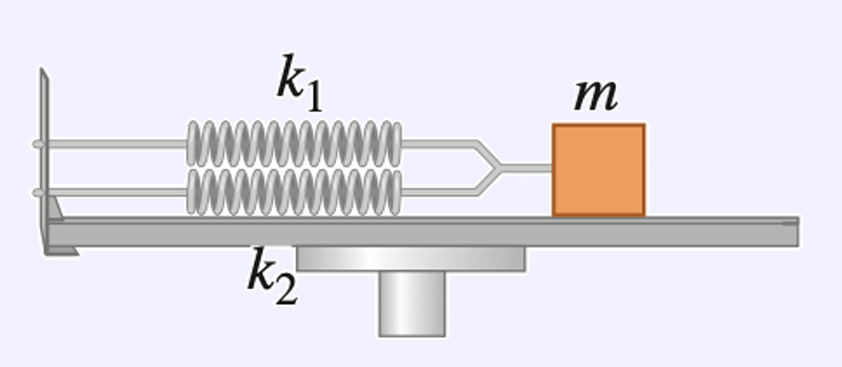
\includegraphics[width=0.3\textwidth]{PB3-a.png}
		\end{center}

		\item[(b)] (10pts)
		\begin{center}
			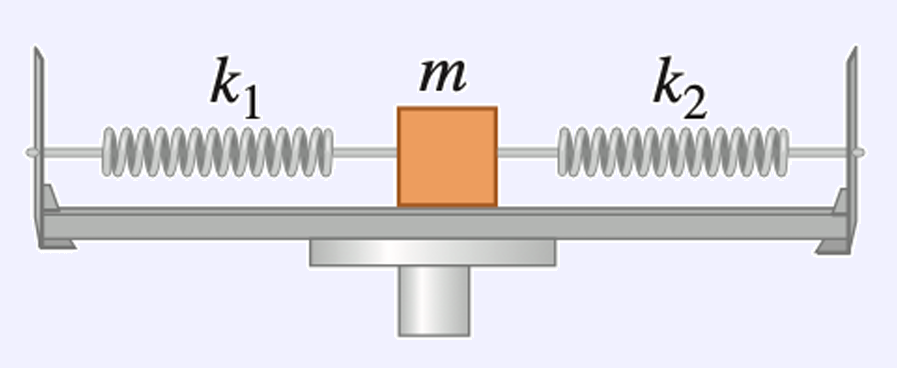
\includegraphics[width=0.3\textwidth]{PB3-b.png}
		\end{center}

		\item[(c)] (10pts)
		\begin{center}
			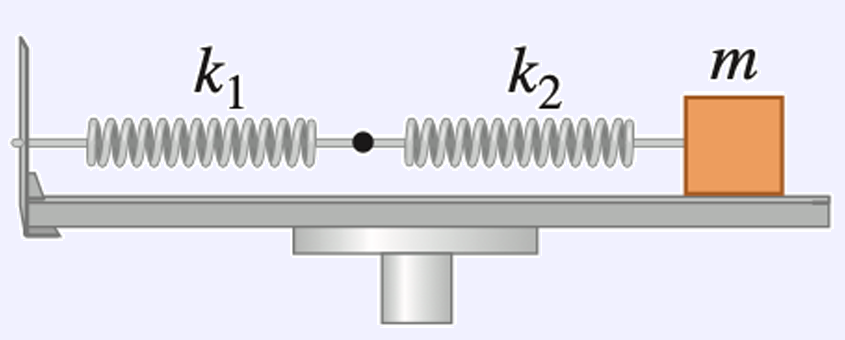
\includegraphics[width=0.3\textwidth]{PB3-c.png}
		\end{center}

		\item[(d)] (10pts) Assume now that you have an object of mass $m$ attached to only one spring with spring constant $k$ and oscillating with frequency $f_1$. If the spring is cut in half and the same object is attached to one of the two halves, its frequency is now $f_2$. What is the ratio $f_2/f_1$?
	\end{enumerate}
\end{problem}

\begin{solution}
	(a) \( F=F_1+F_2=(k_1+k_2)x \), hence \( k_\mathrm{eff}=k_1+k_2 \).\par
	(b) \( F=F_1-F_2=k_1x-k_2(\mathrm{const.}-x)=(k_1+k_2)x+\mathrm{const.} \), hence \( k_\mathrm{eff}=k_1+k_2 \).\par
	(c) \( x=x_1+x_2=F/k_1+F/k_2 \), hence \( k_\mathrm{eff}=k_1k_2/(k_1+k_2) \).\par
	(d) The frequency of oscillation is given by 
	\[ f = \frac{1}{2\pi}\sqrt{\frac{k}{m}}. \]
	When the spring is cut in half, the spring constant of each half becomes \( 2k \) because \( k=(2k)^2/(2k+2k) \). Therefore, the new frequency \( f_2 \) is given by
	\[ f_2 = \frac{1}{2\pi}\sqrt{\frac{2k}{m}}. \]
	The ratio of the frequencies is
	\[ \frac{f_2}{f_1} = \frac{\sqrt{2}}{1} = \sqrt{2}. \]
\end{solution}

\begin{problem}
	(30pts) Consider a one dimensional version of the ``Mexican hat'' potential, which is given by
	\[ U(x)=-\alpha x^2+\beta x^4 \]
	where $\alpha>0$ and $\beta>0$. (A higher-dimensional version of this potential is related to the ``Higgs mechanism'' that is responsible for giving particles a mass and ultimately led to the Nobel Prize in physics in 2013.)
	\begin{enumerate}
		\item[(a)] (10pts) Sketch the potential and determine the location of the local maximum and local minima.
		\item[(b)] (10pts) If you release the particle from the local maximum (by giving it a small perturbation), what is its speed at the local minima? How far does the particle get before turning back?
		\item[(c)] (10pts) Find the period of oscillation for a particle stuck around one of the local minima assuming that $x-x_0$ is small where $x_0$ is the location of the local minimum.
	\end{enumerate}
\end{problem}

\begin{solution}
	(a) The draft of the potential with \( \alpha=\beta=1 \) is shown below. The local maximum is located at \( x=0 \) and the local minima are located at \( x=\pm\sqrt{\alpha/(2\beta)} \).\par
	\begin{figure}[H]
		\centering
		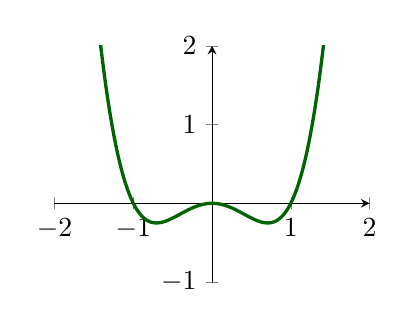
\begin{tikzpicture}[line cap=round,line join=round,>=triangle 45,x=1.0cm,y=1.0cm]
		\begin{axis}[
			x=1.0cm,y=1.0cm,
			axis lines=middle,
			xmin=-2.0,
			xmax=2.0,
			ymin=-1.0,
			ymax=2.0,
			xtick={-2.0,-1.0,...,2.0},
			ytick={-1.0,0.0,...,2.0},]
			\clip(-2.,-1.) rectangle (2.,2.);
			\draw[line width=1.2pt,color=qqwuqq,smooth,samples=100,domain=-2.0:2.0] plot(\x,{0-(\x)^(2.0)+(\x)^(4.0)});
		\end{axis}
		\end{tikzpicture}
	\end{figure}\par
	(b) Suppose the speed of the particle at the local minima is \( v \). Since the particle is released from rest at the local maximum, the total energy of the system is given by \( E = U(0) = 0 \). According to the conservation of energy, we have
	\[ E = E_\mathrm{k} + U(x_0) \implies 0 = \frac{1}{2}mv^2 - \alpha x_0^2 + \beta x_0^4, \]
	where \( x_0=\pm\sqrt{\alpha/(2\beta)} \). Solving for \( v \), we get
	\[ v=\frac{\alpha}{\sqrt{2m\beta}}. \] \par
	Denote the turning point of the particle as \( x_\mathrm{turn} \). At the turning point, the potential energy equals the total energy, hence we have
	\[ U(x_\mathrm{turn}) = 0 \implies -\alpha x_\mathrm{turn}^2 + \beta x_\mathrm{turn}^4 = 0 \implies x_\mathrm{turn}=\sqrt{\alpha/\beta}. \]\par
	(c) The period of oscillation near \( x_0 \) is given by
	\[ T=2\pi \sqrt{\frac{m}{U''(x_0)}}=\pi\sqrt{\frac{m}{\alpha}}. \] 
\end{solution}


\end{document}